\documentclass[10pt]{article} 

\usepackage{fullpage}
\usepackage{bookmark}
\usepackage{amsmath}
\usepackage{amssymb}
\usepackage[dvipsnames]{xcolor}
\usepackage{hyperref} % for the URL
\usepackage{mathtools}
\usepackage[most]{tcolorbox}
\usepackage[amsmath,standard,thmmarks]{ntheorem} 
\usepackage{physics}
\usepackage{tikz}
\usepackage{float}

\usetikzlibrary{shadows}

% floor, ceiling, set
\DeclarePairedDelimiter{\ceil}{\lceil}{\rceil}
\DeclarePairedDelimiter{\floor}{\lfloor}{\rfloor}
\DeclarePairedDelimiter{\set}{\lbrace}{\rbrace}
\DeclarePairedDelimiter{\iprod}{\langle}{\rangle}

\DeclareMathOperator{\Int}{int}
\DeclareMathOperator{\mean}{mean}

% commonly used sets
\newcommand{\R}{\mathbb{R}}
\newcommand{\N}{\mathbb{N}}
\newcommand{\Q}{\mathbb{Q}}
\renewcommand{\P}{\mathbb{P}}

\newcommand{\sset}{\subseteq}

\pagenumbering{gobble}


\begin{document}

\begin{figure}[H]
    \centering
    \tikzset{font=\textbf\footnotesize}
    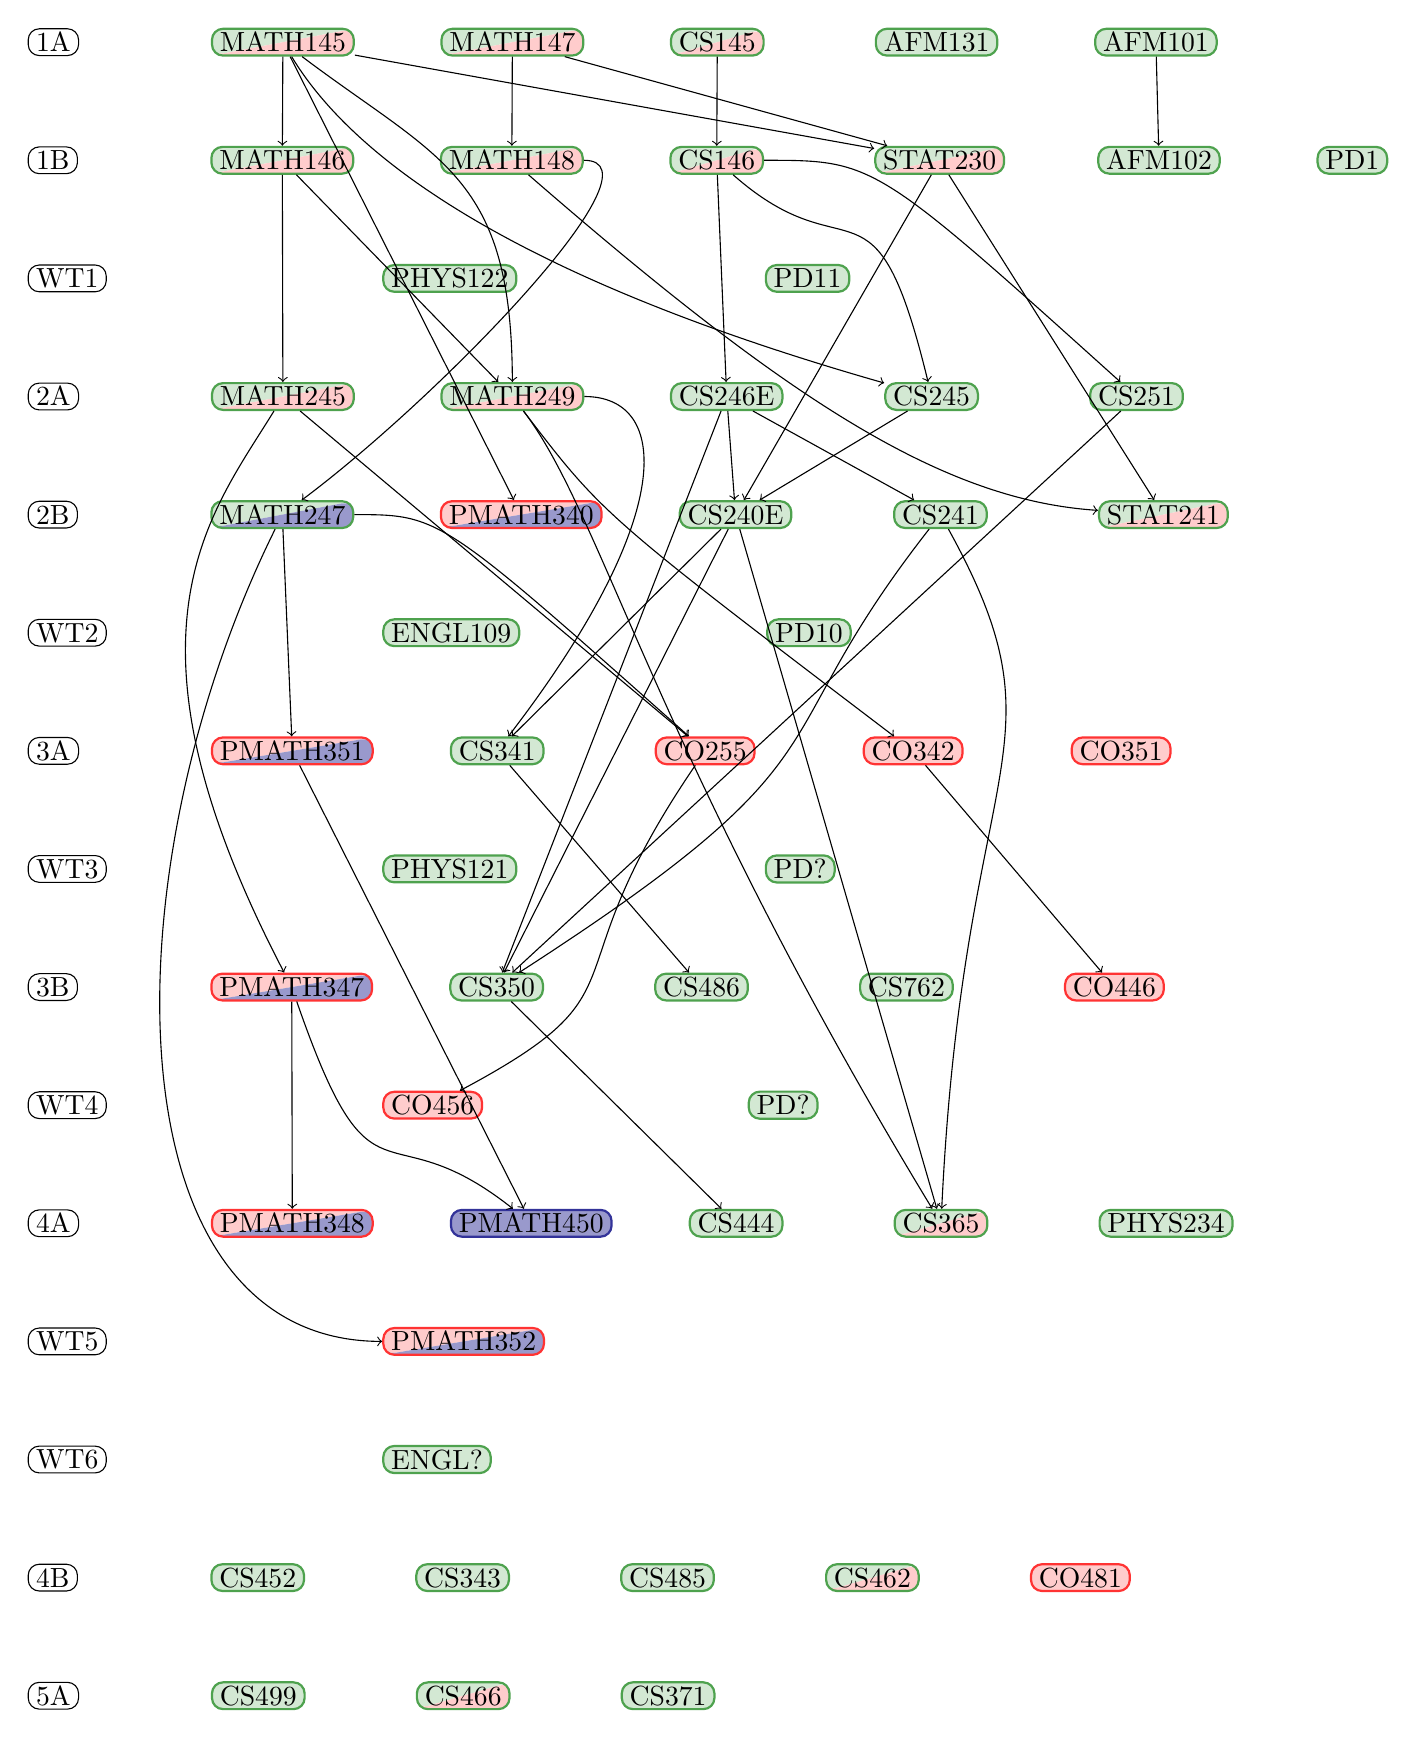
\begin{tikzpicture}[node distance=2cm]
        \tikzstyle{co pm fill}=[path picture={
            \fill[Red!20] (path picture bounding box.south west)
        -- (path picture bounding box.north east) -| cycle;
            \fill[NavyBlue!40] (path picture bounding box.south west)
        -- (path picture bounding box.north east) |- cycle;
        }]
        \tikzstyle{cs pm fill}=[path picture={
            \fill[ForestGreen!20] (path picture bounding box.south west)
        -- (path picture bounding box.north east) -| cycle;
            \fill[NavyBlue!40] (path picture bounding box.south west)
        -- (path picture bounding box.north east) |- cycle;
        }]
        \tikzstyle{cs co fill}=[path picture={
            \fill[ForestGreen!20] (path picture bounding box.south west)
        -- (path picture bounding box.north east) -| cycle;
            \fill[Red!20] (path picture bounding box.south west)
        -- (path picture bounding box.north east) |- cycle;
        }]

        \tikzstyle{basic}=[draw,rectangle,rounded corners,thick,inner xsep=0.1cm,inner ysep=0.5mm]
        \tikzstyle{cs}=[basic,draw=ForestGreen!80,fill=ForestGreen!20]
        \tikzstyle{co}=[basic,draw=Red!80,fill=Red!20]
        \tikzstyle{pm}=[basic,draw=NavyBlue!80,fill=NavyBlue!40]
        \tikzstyle{co pm}=[basic,draw=Red!80,co pm fill]
        \tikzstyle{cs pm}=[basic,draw=ForestGreen!80,cs pm fill]
        \tikzstyle{cs co}=[basic,draw=ForestGreen!80,cs co fill]
        \tikzstyle{term}=[basic,thin]

        \tikzstyle{prereq}=[<-,thin]

        \begin{scope}[node distance=4cm]
            \node[term,alias=last,anchor=west] (WT1) at (0, -3) {WT1};
            \foreach \title/\style in {PHYS122/cs,PD11/cs} {
                \node (\title) [\style,right of=last,alias=last,anchor=west] {\title};
            }

            \node[term,alias=last,anchor=west] (WT2) at (0, -7.5) {WT2};
            \foreach \title/\style in {ENGL109/cs,PD10/cs} {
                \node (\title) [\style,right of=last,alias=last,anchor=west] {\title};
            }

            \node[term,alias=last,anchor=west] (WT3) at (0, -10.5) {WT3};
            \foreach \title/\style in {PHYS121/cs,PD?/cs} {
                \node (\title) [\style,right of=last,alias=last,anchor=west] {\title};
            }
            
            \node[term,alias=last,anchor=west] (WT4) at (0, -13.5) {WT4};
            \foreach \title/\style in {CO456/co,PD?/cs} {
                \node (\title) [\style,right of=last,alias=last,anchor=west] {\title};
            }

            \node[term,alias=last,anchor=west] (WT5) at (0, -16.5) {WT5};
            \foreach \title/\style in {PMATH352/co pm} {
                \node (\title) [\style,right of=last,alias=last,anchor=west] {\title};
            }

            \node[term,alias=last,anchor=west] (WT6) at (0, -18) {WT6};
            \foreach \title/\style in {ENGL?/cs} {
                \node (\title) [\style,right of=last,alias=last,anchor=west] {\title};
            }
        \end{scope}

        \node[term,alias=last,anchor=west] (1A) at (0, 0) {1A};
        \foreach \title/\style in {MATH145/cs co,MATH147/cs co,CS145/cs co,AFM131/cs,AFM101/cs} {
            \node (\title) [\style,right of=last,alias=last,anchor=west] {\title};
        }

        \node[term,alias=last,anchor=west] (1B) at (0, -1.5) {1B};
        \foreach \title/\style in {MATH146/cs co,MATH148/cs co,CS146/cs co,STAT230/cs co,AFM102/cs,PD1/cs} {
            \node (\title) [\style,right of=last,alias=last,anchor=west] {\title};
        }

        \draw[prereq] (MATH146) -- (MATH145);
        \draw[prereq] (MATH148) -- (MATH147);
        \draw[prereq] (CS146) -- (CS145);
        \draw[prereq] (STAT230) -- (MATH145);
        \draw[prereq] (STAT230) -- (MATH147);
        \draw[prereq] (AFM102) -- (AFM101);

        \node[term,alias=last,anchor=west] (2A) at (0, -4.5) {2A};
        \foreach \title/\style in {MATH245/cs co,MATH249/cs co,CS246E/cs,CS245/cs,CS251/cs} {
            \node (\title) [\style,right of=last,alias=last,anchor=west] {\title};
        }

        \draw[prereq] (MATH245) -- (MATH146);
        \draw[prereq] (MATH249) .. controls (MATH148.south) and (MATH148.west) .. (MATH145);
        \draw[prereq] (MATH249) -- (MATH146);
        \draw[prereq] (CS246E) -- (CS146);
        \draw[prereq] (CS245) .. controls (STAT230.west) and (PD11.east) .. (CS146);
        \draw[prereq] (CS245) .. controls (PHYS122.east) and (MATH146.east) .. (MATH145);
        \draw[prereq] (CS251) .. controls (STAT230.west) .. (CS146);

        \node[term,alias=last,anchor=west] (2B) at (0, -6) {2B};
        \foreach \title/\style in {MATH247/cs pm,PMATH340/co pm,CS240E/cs,CS241/cs,STAT241/cs co} {
            \node (\title) [\style,right of=last,alias=last,anchor=west] {\title};
        }

        \draw[prereq] (MATH247) .. controls (MATH249.west) and (CS146.west) .. (MATH148);
        \draw[prereq] (PMATH340) -- (MATH145);
        \draw[prereq] (CS240E) -- (CS245);
        \draw[prereq] (CS240E) -- (CS246E);
        \draw[prereq] (CS240E) -- (STAT230);
        \draw[prereq] (CS241) -- (CS246E);
        \draw[prereq] (STAT241) -- (STAT230);
        \draw[prereq] (STAT241) .. controls (CS241.north) and (CS246E.east) .. (MATH148);

        \node[term,alias=last,anchor=west] (3A) at (0, -9) {3A};
        \foreach \title/\style in {PMATH351/co pm,CS341/cs,CO255/co,CO342/co,CO351/co} {
            \node (\title) [\style,right of=last,alias=last,anchor=west] {\title};
        }

        \draw[prereq] (PMATH351) -- (MATH247);
        \draw[prereq] (CS341) -- (CS240E);
        \draw[prereq] (CS341) .. controls (CS240E.west) and (CS246E.west) .. (MATH249);
        \draw[prereq] (CO255) -- (MATH245);
        \draw[prereq] (CO255) .. controls (PMATH340.west) .. (MATH247);
        \draw[prereq] (CO342) .. controls (PMATH340.east) .. (MATH249);

        \node[term,alias=last,anchor=west] (3B) at (0, -12) {3B};
        \foreach \title/\style in {PMATH347/co pm,CS350/cs,CS486/cs,CS762/cs,CO446/co} {
            \node (\title) [\style,right of=last,alias=last,anchor=west] {\title};
        }

        \draw[prereq] (PMATH347) .. controls (WT2.east) and (MATH247.west).. (MATH245);
        \draw[prereq] (CS350) -- (CS240E);
        \draw[prereq] (CS350) .. controls (CO342.west) and (CO255.east).. (CS241);
        \draw[prereq] (CS350) -- (CS246E);
        \draw[prereq] (CS350) -- (CS251);
        \draw[prereq] (CS486) -- (CS341);
        \draw[prereq] (CO446) -- (CO342);

        \draw[prereq] (CO456) .. controls (CS486.west) and (CS350.east) .. (CO255);

        \node[term,alias=last,anchor=west] (4A) at (0, -15) {4A};
        \foreach \title/\style in {PMATH348/co pm,PMATH450/pm,CS444/cs,CS365/cs co,PHYS234/cs} {
            \node (\title) [\style,right of=last,alias=last,anchor=west] {\title};
        }

        \draw[prereq] (PMATH348) -- (PMATH347);
        \draw[prereq] (PMATH450) .. controls (CO456.west) and (PMATH348.east) .. (PMATH347);
        \draw[prereq] (PMATH450) -- (PMATH351);
        \draw[prereq] (CS444) -- (CS350);
        \draw[prereq] (CS365) -- (CS240E);
        \draw[prereq] (CS365) .. controls (CO342.east) and (CO351.west) .. (CS241);
        \draw[prereq] (CS365) .. controls (CO255.west) and (PMATH340.east) .. (MATH249);

        \draw[prereq] (PMATH352) .. controls (WT5.east) and (WT3.east) .. (MATH247);

        \node[term,alias=last,anchor=west] (4B) at (0, -19.5) {4B};
        \foreach \title/\style in {CS452/cs,CS343/cs,CS485/cs,CS462/cs co,CO481/co} {
            \node (\title) [\style,right of=last,alias=last,anchor=west] {\title};
        }

        \node[term,alias=last,anchor=west] (5A) at (0, -21) {5A};
        \foreach \title/\style in {CS499/cs,CS466/cs co,CS371/cs} {
            \node (\title) [\style,right of=last,alias=last,anchor=west] {\title};
        }
    \end{tikzpicture}
\end{figure}

\end{document}
